\chapter{Aufgaben im Labor}
\thispagestyle{fancy}

\section{Theoretische Lösung aus V1 (A1)}

\textbf{Aufgabenstellung:\\}
Schreiben Sie ein Programm, das die theoretische Lösung aus V1 für 1 t = T zeigt, d.h. die Ausgangsspannung $u_y(t)$ t . Stellen Sie das Bild für 0 <= t <= T + 5$\tau$ dar. Verwenden Sie dazu den "plot" - Befehl. Beschriften Sie den Plot mit Hilfe von \textbf{title} und \textbf{xlabel}.

\vspace{1.5cm}

\begin{lstlisting}
%% Aufgabe 1

% Berechnung der Lade- und Entladekurve

t1 = 0:dt:tau;              % Ladezeit
uy1 = U * (1-exp(-t1/tau)); % Ladefunktion

t2 = tau:dt:(tau+5*tau);    % Entladezeit
uy2 = U * (1-exp(-tau/tau)) * exp(-(t2-tau)/tau); % Entladefkt

uy = [uy1, uy2];    % Zusammensetzen der Lade- und Entladewerte
t = [t1, t2];

plot(t, uy); grid on; grid minor; %axis tight; 

% Beschriftung des Graphen:

title('Ausgangsspannung u_y(t)');
xlabel('t');
ylabel('u_y(t)');

\end{lstlisting}

\vspace{0.5cm}

\newpage
    
    
Ausgegeben wird folgende Grafik:
\begin{center}
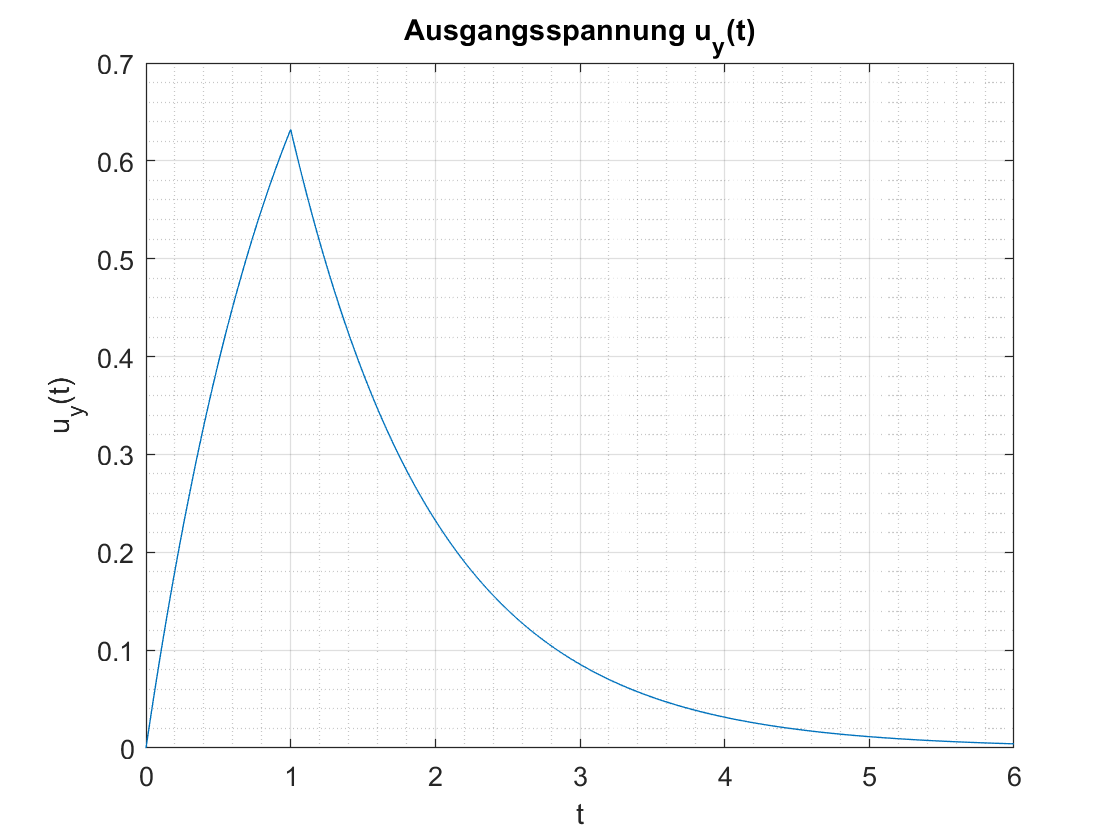
\includegraphics[width=300pt]{img/aufgabe1.png}
\end{center}

\vspace{0.7cm}

\section{Erweiterung der ersten Aufgabe (A2)}

\textbf{Aufgabenstellung:\\}
Nun soll 1 t = m*T/5 mit m = 1,…,10 gelten. Erweitern Sie das Skript um eine Schleife über m, die mit \textbf{pause} zum Ansehen angehalten wird. Beschriften Sie den Plot mit Hilfe von \textbf{title}, \textbf{xlabel} und \textbf{num2str}. Speichern Sie die Bilder für m = 1,3, und 10 ab.

\vspace{1.5cm}

\begin{lstlisting}
%% Aufgabe 2
U = 1; 
T1 = 1; % Umschaltzeitpunkt
tau = 1; 
dt = tau/100;

for m = 1:10
	tau = m*T1/5;
	
	t1 = (0:dt:T1);
	uy1 = U * (1-exp(-t1/tau));
	
	t2 = (T1:dt:((T1+5*tau)));
	uy2 = U * (1-exp(-T1/tau)) * exp(-(t2-T1)/tau);
	uy = [uy1 uy2];
	
	t = [t1 t2];
	
	if (m == 1 || m == 3 || m == 10)
		plot(t, uy);
		legend(strcat('m = ', num2str(m)));
		hold on;
	end
	
	pause(0.5);	
end
	
% Beschriftung des Plots
title('Ausgangsspannung u_y(t)');
legend('m = 1', 'm = 3', 'm = 10');
xlabel('t');
ylabel('u_y(t)');

grid on; grid minor; axis tight; % Optimierung Graph
\end{lstlisting}

\vspace{1cm}

Ausgegeben wird folgende Grafik:

\begin{center}
	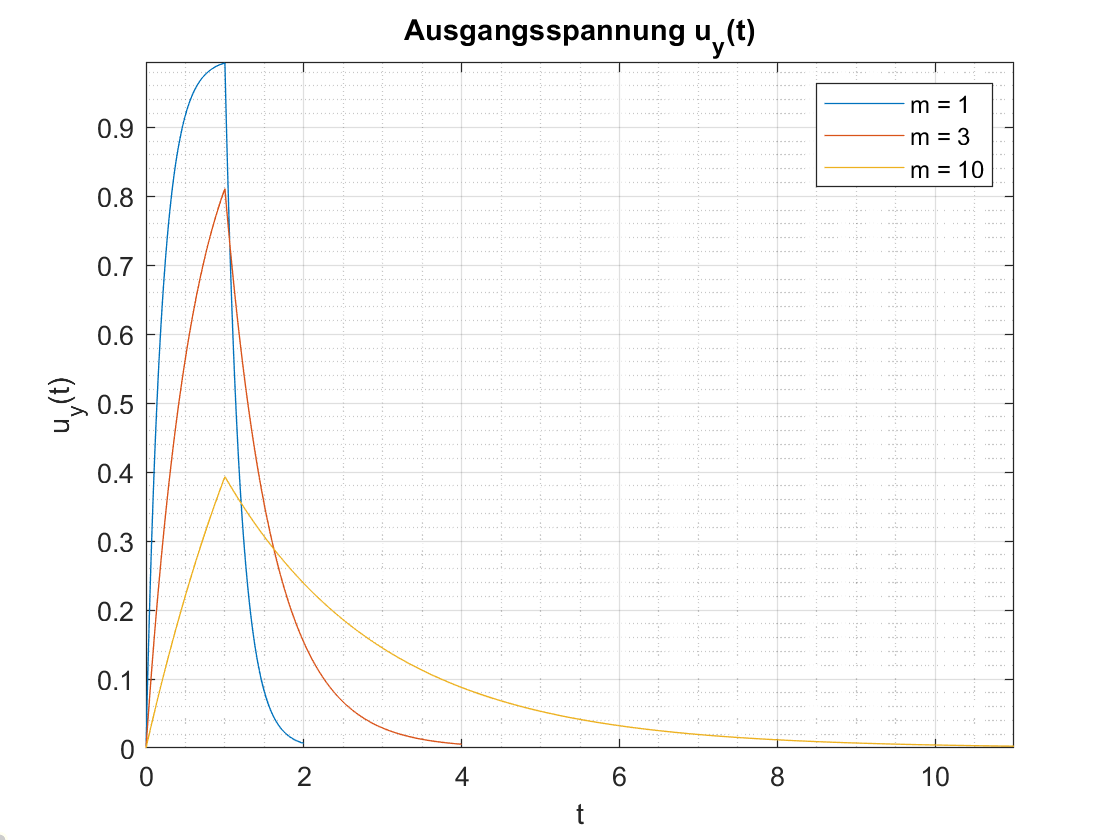
\includegraphics[width=300pt]{img/aufgabe2.png}
\end{center}

Je größer m ist, desto langsamer steigt die Spannung am Kondensator. Somit kann m als Dämpfungsfaktor angesehen werden. Physikalisch ist m der Multiplikator des Widerstandes in der RC-Schaltung.

\newpage

\section{Approximation der Lade- und Entladekurve (A3)}

\textbf{Aufgabenstellung:\\}
Es gilt wieder 1 t = T . Approximieren Sie $u_y(t)$ , indem Sie die Fourierreihe mit den Koeffizienten k Y mit −K£ k £K berechnen. Schreiben Sie eine Schleife über K und sehen Sie sich die Bilder für K = 1,…, 40 an. Speichern Sie sinnvoll 3 Bilder ab. Beschriften Sie die Bilder analog zu A2.

\vspace{0.5cm}

\begin{lstlisting}
%% Aufgabe 3

T = 5;  % Periodendauer
tau = 1;
t1 = linspace(0, tau, 1000);
t2 = linspace(tau, 4*tau, 4000);
F = 1/T;
t = [t1, t2];
dt = tau/100;

% Berechnung der Fourier-Reihe
for K = 1:40
	uyt = 0;
	
	for k = -K:K
		Hkf = 1 / (1 + 1i*2*pi*k*F*tau);
		Xk = exp(-1i*2*pi*k*F*(tau/2)) * (tau/T) * sinc(k*F*tau); %% sinc ohne PI!
		Yk = Hkf * Xk;
		uyt = uyt + Yk * exp(1i*2*pi*k*F*t);
	end
	if (K == 2 || K == 12 || K == 40)
		plot(t, uyt);
		legend(strcat('K = ', num2str(K))); % Ausgabe des k-ten Durchlauf
		hold on;
	end
	%pause(0.2);
end
% Beschriftung des Plots
	
title('Fourier-Reihe u_y(t) mit K_{max} = 40' );
xlabel('t');
ylabel('u_y(t)');
legend('K = 2', 'K = 12', 'K = 40');
grid on; grid minor;
	
hold off;
\end{lstlisting}

\newpage

Ausgegeben wird folgende Grafik:

\begin{center}
	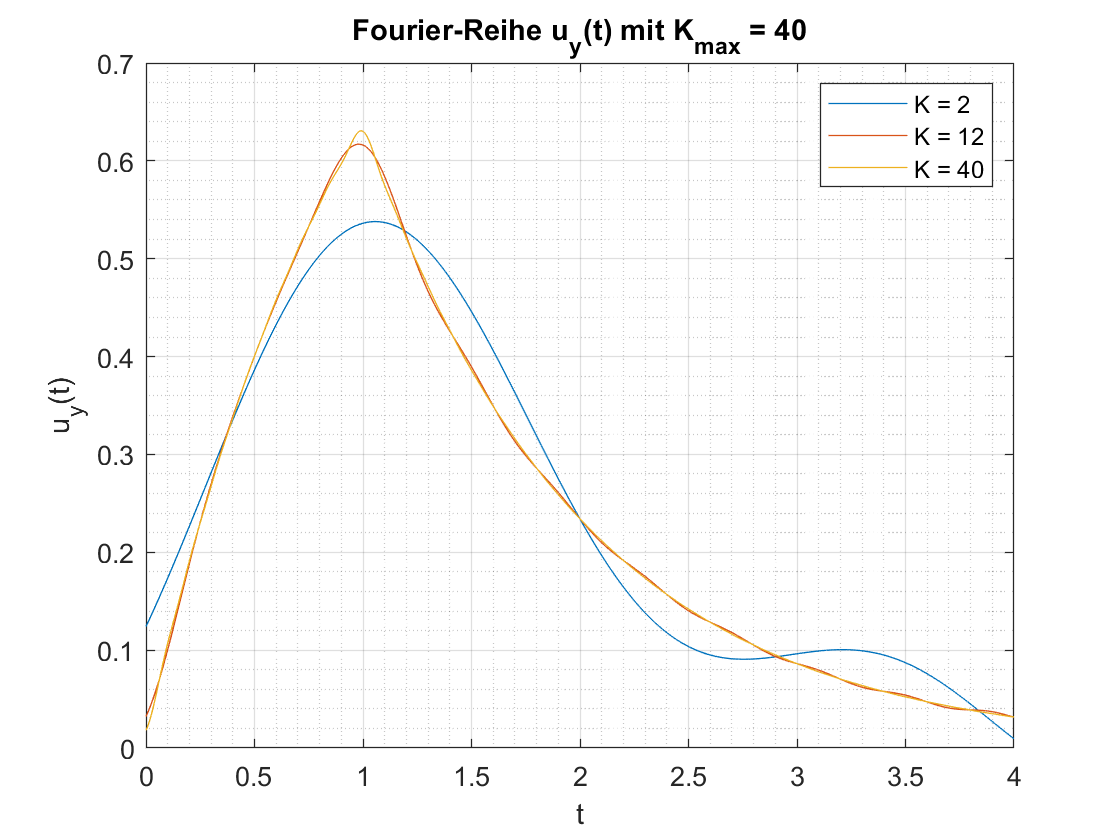
\includegraphics[width=300pt]{img/aufgabe3.png}
\end{center}

Wie zu erwarten nähert sich die approximierte Funktion mit steigenden K der theoretischen Funktion an. Bei K = 40 ist kaum noch ein unterschied zu erkennen.